La gerarchia vuole modellare degli oggetti che comprendono tutti i file audio-visivi ed è così composta: una classe base astratta denominata \texttt{AudioVisual} e tre classi derivate concrete \texttt{TvSerie}, \texttt{Movie}, \texttt{Documentary} che implementano i metodi puri della classe base. 

\begin{center}
    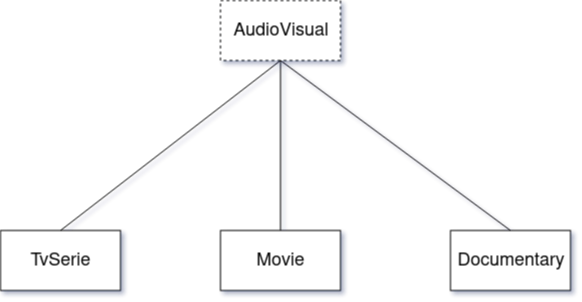
\includegraphics[width=0.6\textwidth]{gerarchia}
\end{center}

\paragraph{AudioVisual}
La classe base della gerarchia fornisce le informazioni di base comuni a tutti i file di tipo audio-visivo, ossia il \textit{titolo} del file, l'\textit{immagine} di copertina, la \textit{descrizione} della trama, la \textit{data} di rilascio espressa in anni, la \textit{durata} in minuti, il nome del \textit{regista}, se il file appartiene ai \textit{preferiti} dell'utente, se l'audio è \textit{compresso} o meno, la \textit{risoluzione} dell'immagine, i \textit{frame per secondo}.

\paragraph{TvSerie}
TvSerie è una classe derivata concreta che rappresenta i file riguardanti le serie tv, infatti aggiunge i campi dati riguardanti il numero di \textit{episodi} della serie, il numero di \textit{stagioni}, se la serie è \textit{terminata}, il \textit{rating}, il \textit{genere}, il \textit{cast} formato dai personaggi.

\paragraph{Documentary}
Documentary è una classe derivata concreta che rappresenta i file di tipo documentario, in cui si ha un \textit{topic} che spazia dall'argomento scientifico, a quello storico o biografico e un campo dati riservato al \textit{narratore}.

\paragraph{Movie}
Movie è anch'essa una classe derivata concreta che vuole rappresentare i file di tipo film; aggiunge i campi dati riguardanti il \textit{cast}, il \textit{rating} ed il \textit{genere}. \newline

La gerarchia attuale è stata pensata per essere estensibile in futuro, sia in orizzontale, per esempio implementando una classe riguardante i video di YouTube, che in vertiale, per esempio derivando da \texttt{TvSerie} una classe che rappresenti le telenovelas. \newline
Inoltre non fa uso di dati o classi riguardanti il framework QT, per cui è indipendente da esso.

\paragraph{DeepPtr}
Il progetto fa uso anche di un template di classe \texttt{DeepPtr<T>} di puntatori polimorfi al tipo T che implementano la gestione automatica della memoria cosidetta profonda. È quindi necessario che ogni classe concreta della gerarchia implementi il metodo relativo alla clonazione e anche la distruzione polimorfa.

\paragraph{Polimorfismo}
All'interno della gerarchia, nella classe base, sono stati dichiarati 5 metodi virtuali puri che vengono poi implementati nelle classi derivate concrete. 
\begin{enumerate}
    \item \texttt{virtual AudioVisual* clone() const =0;} utilizzato dallo \textit{SmartPointer} per la copia profonda dell'oggetto.
    \item \texttt{virtual unsigned int getTotalRunningTime() const =0;} che si occupa di calcolare la durata totale di ogni oggetto.
    \item \texttt{virtual std::string getType() const =0;} restituisce sottoforma di stringa il tipo dell'oggetto.
    \item \texttt{virtual bool isHighQuality() const =0;} che determina se un oggetto è di qualità o meno in base alla risoluzione dell'immagine, della compressione dell'audio e dei frame per secondo.
    \item \texttt{virtual bool matureContent() const =0;} si occupa di determinare se l'oggetto è visionabile solo da adulti.
\end{enumerate}
Inoltre, sebbene non siano metodi puri, sono stati dichiarati virtuali anche i metodi \texttt{virtual bool operator==(const AudioVisual\&) const;} che fa un confronto tra ogni campo dati presente nella classe e anche il distruttore.




%4k, 144p, 240, 480, 360, 720
%4k/2160p, FullHD/1080p, HD/720p, SD/480p, LD/240p
